\documentclass[english]{article}
\usepackage[T1]{fontenc}
\usepackage[utf8]{inputenc}
\usepackage{babel}
\usepackage{graphicx}
\usepackage{caption}
\usepackage{subcaption}
\usepackage{listings}

\newcommand{\design}{Nengo-RT}

\begin{document}

\lstset{basicstyle=\footnotesize}

\section{Introduction}

\subsection{Motivation}

\subsection{Potential Applications}

\subsection{State of the Art (Neuromorphic Hardware)}

\section{Methods}

\subsection{Description of NEF and population mode}

\subsubsection{Considerations related to hardware (multiplexing, clustering, using principal components)}

% FIXME brief description of FPGA hardware and programming

\subsection{High-level system description}

\design{} is a custom digital hardware design that implements the population-mode NEF in real-time (1~ms timestep).
A block diagram of the design is shown in Figure~\ref{fig:system}.
The encoder units perform the function of encoding (), % FIXME NEF equation
while the population units perform the decoding () % FIXME NEF equation
and write the decoded values to the decoded value buffers
to be used as inputs to other populations or as outputs from the network.
Each population of neurons is assigned to a population unit, which is able to simulate up to 1024 populations
having either one or two encoded inputs each. These inputs are calculated by the encoder units,
of which there are two for a one-dimensional population unit and four for a two-dimensional population unit;
each encoder unit can be associated with a different first-order filter to simulate post-synaptic filtering.
For example, one of the two encoders on a one-dimensional population unit can be programmed with
a small time constant to model fast synapses (e.g. AMPA and GABA$_A$), while the second can be programmed
with a large time constant to model slow synapses (e.g. NMDA and GABA$_B$).
Each population unit performs time-multiplexing and swaps in different sets of decoders
in order to run more populations on the same hardware. The principal components are fixed and must be shared
between all populations on an individual population unit.
Each population unit writes to a fixed set of decoded value buffers, but a shared interconnect
allows the encoder units to perform random accesses to these buffers.
This allows effective all-to-all communication between populations while reducing the number of 
connections that must be made between population units.
A number of decoded value buffers are reserved for external inputs to the network,
which can be sent from the controlling computer system over an Ethernet connection.
The output channels can also be programmed to send decoded values back to the computer over Ethernet.

\begin{figure}
\centering

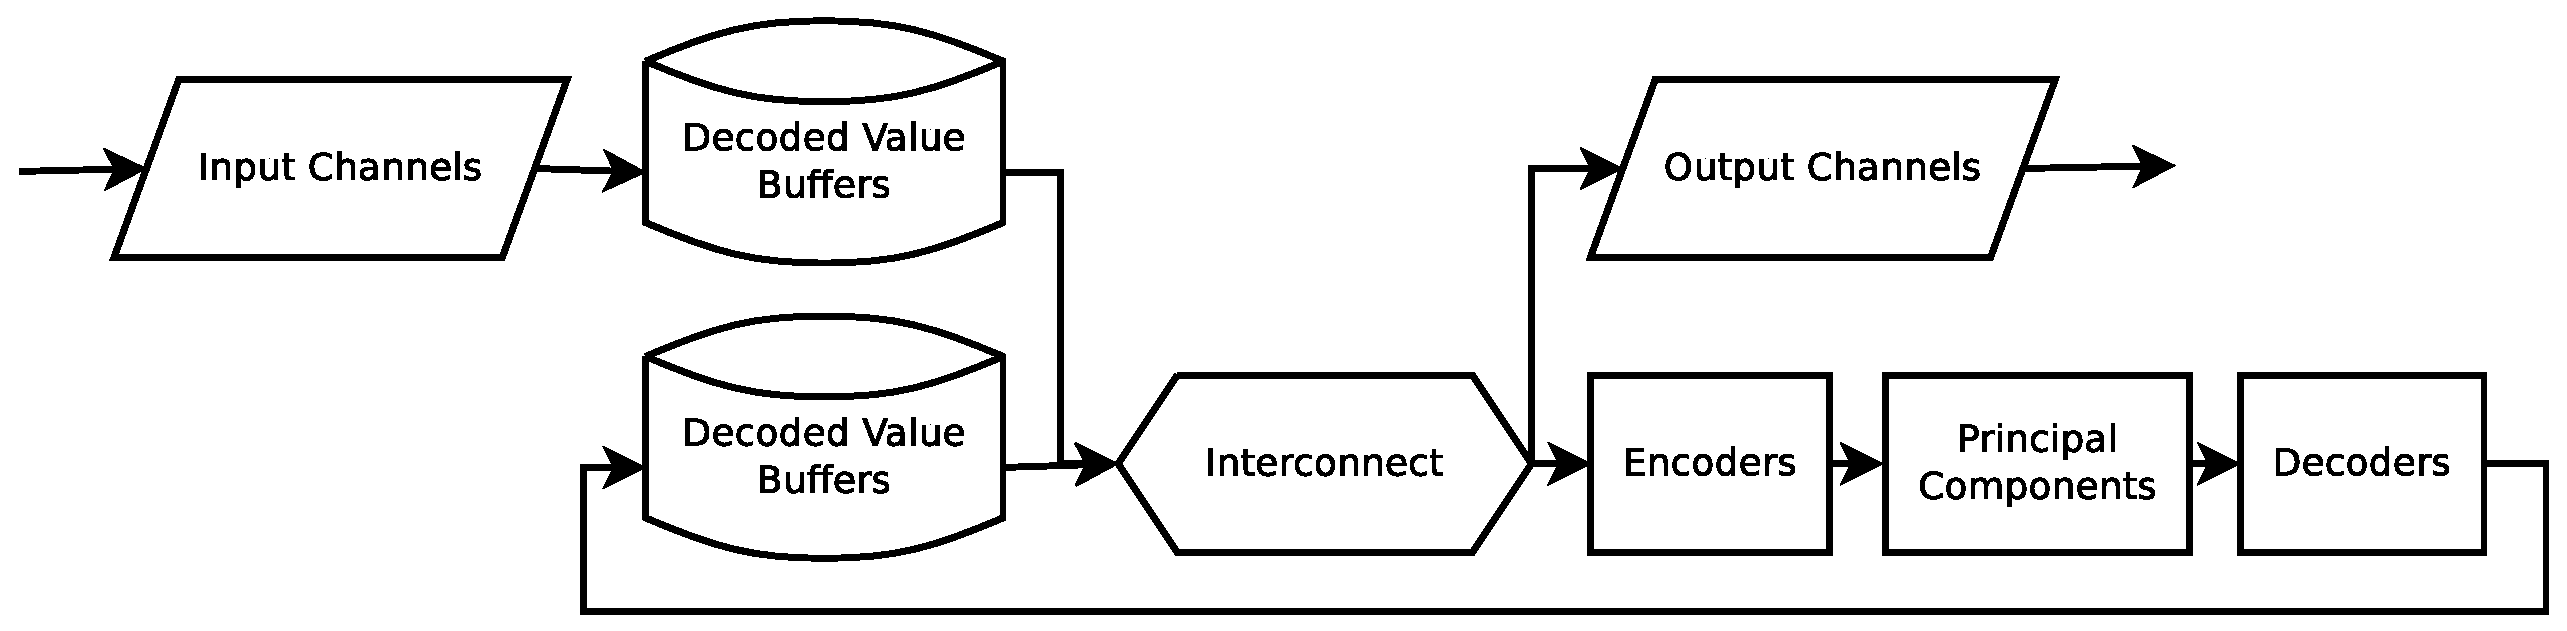
\includegraphics[width=6in]{system-block-diagram.eps}

\caption{Block diagram of the \design{} hardware design.}

\label{fig:system}
\end{figure}

\subsection{Hardware design details}

\subsubsection{Encoder Unit}

It is too resource-intensive to create a connection from the output of each population unit to the inputs of all population units (including itself).
In order to allow communication of information across population units, the decoded values from each population are stored in a local buffer.
Then, every population unit has a number of encoder units that are responsible for reading decoded values from each buffer. 
Each encoder unit communicates with the decoded value buffers over a shared interconnect, described below.
A maximum of two encoder units are allowed to access a single decoded value buffer simultaneously
without causing a bus collision, since the memory primitives used to implement the buffers have two independent read ports.

Each encoder unit is attached to a circular buffer of size 8192
containing a list of instructions for calculating one encoded value. 
This size was chosen as a compromise between memory utilization and encoder flexibility;
it means that a single population can have a maximum fan-in of eight connections (including connections from the population to itself).
To execute an instruction, the encoder sends the decoded value address it wants to read from to the interconnect
and then reads the corresponding decoded value on its data input port three clock cycles later.
The value is then multiplied by a fixed-point weight, which is given as part of the instruction field, and added to an accumulator in the encoder.
The interconnect is responsible for routing address and value data between the encoders and the buffers.
A portion of the instruction field provides a delay (expressed as a number of clock cycles) to the encoder before executing this instruction.
This is necessary when many encoders are accessing the interconnect simultaneously in order to prevent too many of them from reading
from the same buffer at the same time (which would result in data corruption, because only two concurrent accesses are possible).
A certain bit in the instruction field acts as a flag to indicate that the encoded value is ready to be passed on to the population unit after this
instruction finishes executing. The encoder unit then waits for all other encoders to finish in order to synchronize
access to the shared interconnect, then resets the accumulator and begins encoding the next value.
To synchronize encoders across population units, a single encoding controller connects to all encoder units and is responsible for
signalling them to start encoding when it detects that they have all finished encoding the previous value.

\subsubsection{Population Unit}

Encoded values are passed from the encoder units to the population units. 
Population units are either one-dimensional or two-dimensional.
This means the groups of neurons they model have firing rates that are static functions of either a one- or two-dimensional represented variable.
Both types of population unit receive input from two encoder units in each input dimension;
for each dimension, the encoded values are passed through a first-order filter which performs post-synaptic filtering,
and are then summed. The value resulting from this operation is
truncated to the most significant 10 bits and is then used as input to a set of lookup tables,
implemented as a bank of synchronous RAM elements. SRAMs are used
because the contents of these tables are not known until simulation-time and therefore the lookups cannot be implemented as hardware logic functions.
Each lookup table contains the 12-bit fixed-point values of points sampled from 
principal components of the spike rates of neurons in a population, as a function of the variable that the population encodes.
In order to reduce the amount of memory used by each population, all populations on a population unit must share principal components.
For one-dimensional population units, there are seven such lookup tables, and each one contains
1024 values sampled at equally-spaced points on the open interval $(-2, 2)$. For two-dimensional population units,
there are fifteen lookup tables, each containing 1024 values sampled at equally-spaced points on a square of width 4
centered at $(0, 0)$. The resulting sample space is a 32x32 grid.
These numbers of principal components account for most of the variation in spike rates across 1D and 2D populations.
% FIXME find out exactly how much of this variation they account for over random populations with a variety of parameters, and mention this.
To increase the accuracy of this representation, each two-dimensional population unit performs bilinear interpolation
using the least significant five bits of each input variable to determine the distance between sample points. 
The extra resources used to perform this operation are modest
and significantly reduce the amount of memory used for two-dimensional populations while maintaining a good degree of accuracy of representation.

To simulate the noise resulting from a neural representation, a pseudorandom Gaussian noise generator is implemented in each population unit.
The output from the noise generator is passed through a pre-defined second-order filter to approximate the power spectrum of the noise
that would be present if individual neurons were being implemented. % FIXME for completeness, give the transfer function

The interpolated values from the principal component lookup tables and the filtered noise sample are multiplied by a vector of decoders,
and these results are summed to produce a decoded value. % FIXME refer to equations
One of the decoders corresponds to a gain term that can be used to control the amplitude of the noise.
Each population unit can store up to four independent sets of decoders per population being simulated,
which allows each population to produce a maximum of four decoded values as some function of its inputs
(and the resulting values of its principal components).

\subsubsection{Decoded Value Buffers and Interconnect}

Decoded values calculated from population units are stored in decoded value buffers, which are fairly large memory banks that can each
store 2048 decoded values. 
Because each population unit produces 4096 decoded values (1024 DVs from each of four decoder vectors),
this means that a population unit must be attached to the write ports of two separate decoded value buffers.
The buffers themselves expose a read-only interface, accessed by the encoders to read decoded values from the
previous timestep, and a write-only interface, accessed by the population units when new decoded values are calculated.
Internally, each interface is connected to a separate dual-port RAM; the connections are swapped between RAMs
at the end of each timestep in order to implement double-buffering, so that it is not possible for encoders to read a
partially-updated set of decoded values, where some are from the previous timestep and some are freshly written during the current timestep.
A diagram of this component is shown in Figure~\ref{fig:dvdoublebuffer}.
The reason for choosing a size of 2048 is because of this implementation detail; on the particular family of hardware
that was used to implement the prototype, the largest single-component 12-bit dual-port RAM available has space for 1024 words,
and two separate RAM components are necessary in order to implement the double buffer, hence a total size of 2048 words of memory.

\begin{figure}
\centering

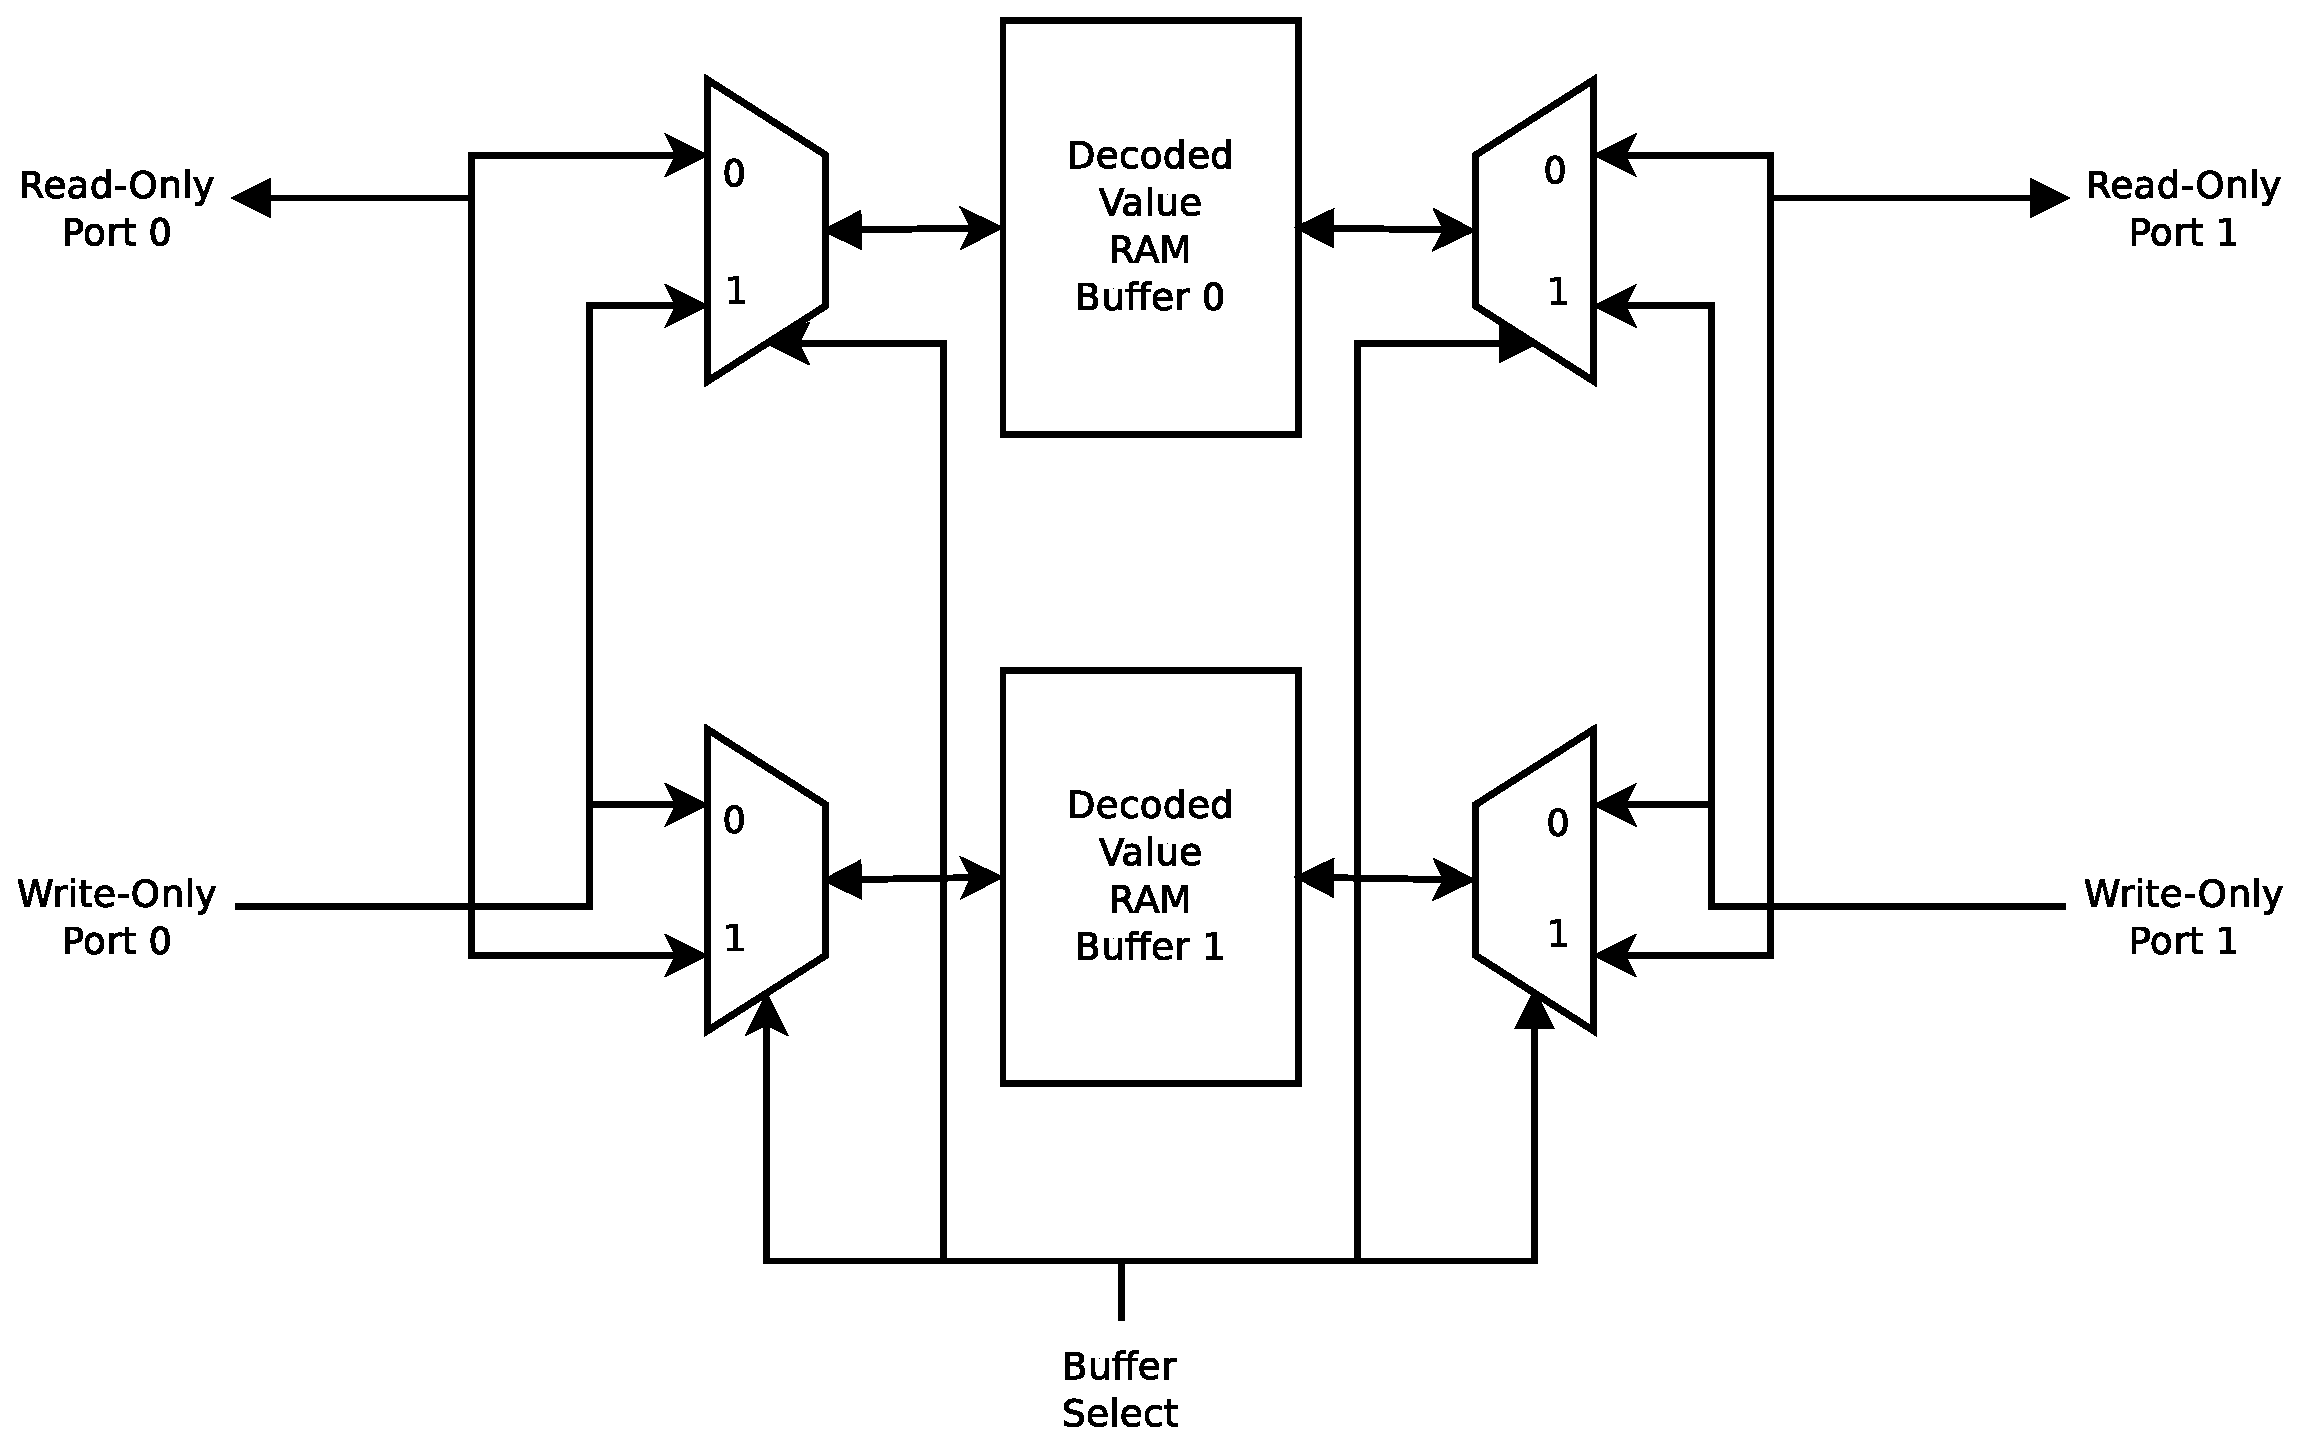
\includegraphics[width=6.0in]{dv-double-buffer-diagram.eps}

\caption{Block diagram of the decoded value double-buffer component.}
\label{fig:dvdoublebuffer}
\end{figure}

The encoders must share access to the read-only interface of the decoded value buffers. To accomplish this,
the encoders are connected to the decoded value buffers over a shared interconnect. Access to the decoded value buffers
is managed by arbiters that inspect the addresses requested by encoders and redirect the read operations to the
corresponding buffers. A maximum of two encoders may be accessing a single buffer at any one time.
Therefore, it is up to the compiler to generate a sequence of read instructions for the encoders that ensures that this
constraint is respected. The delay field in the encoder instruction word can be used for this purpose to make an encoder
wait until another is finished with its access before attempting to read from the same buffer.

\subsubsection{Input, Output, and Control}

A number of decoded value buffers, which can be customized at the time the hardware is synthesized
(but always at least one)
are set aside for use as inputs to the simulation. These are indistinguishable from other decoded value buffers
from the perspective of the encoders and interconnect, but instead of being written to by population units,
they are connected to one or more input channels which are responsible for receiving data from an external source
and writing it to the buffers.

To provide output to an external source, such as a simulation GUI running on a computer, one or more output channels
are made accessible on the hardware. The exact number of output channels, as well as their features, will depend on the hardware used to implement the design.
The function of the output channel is to read from the decoded value buffers and output the desired decoded values to be transmitted
to an external device. Output channels do not have access to the interconnect until all encoders have finished all
encoding operations for this timestep. At that point, the encoders are detached from the interconnect by a separate controller and the output
channels are attached in their place. This allows the output channels to share interconnect logic with the encoders;
it also increases efficiency both by reducing contention on the shared interconnect (as the encoders and output channels
do not access it at the same time) and by allowing output to happen at the same time as decoding
(the double-buffering of decoded values means that output channels always see a consistent set of values,
so these operations can be performed in parallel).

Both the input and output channels are transport-agnostic and can be attached to application-specific custom hardware that allows for
I/O to be performed over the desired interface, such as Ethernet. The implemented design performs I/O over Gigabit Ethernet using a custom Ethernet frame format for efficiency.
Input and output channels could also be implemented for sensors and actuators to allow for autonomous operation of a Nengo network in hardware once it has been sent to the board
(Figure~\ref{fig:closedloop}).

\begin{figure}
\centering

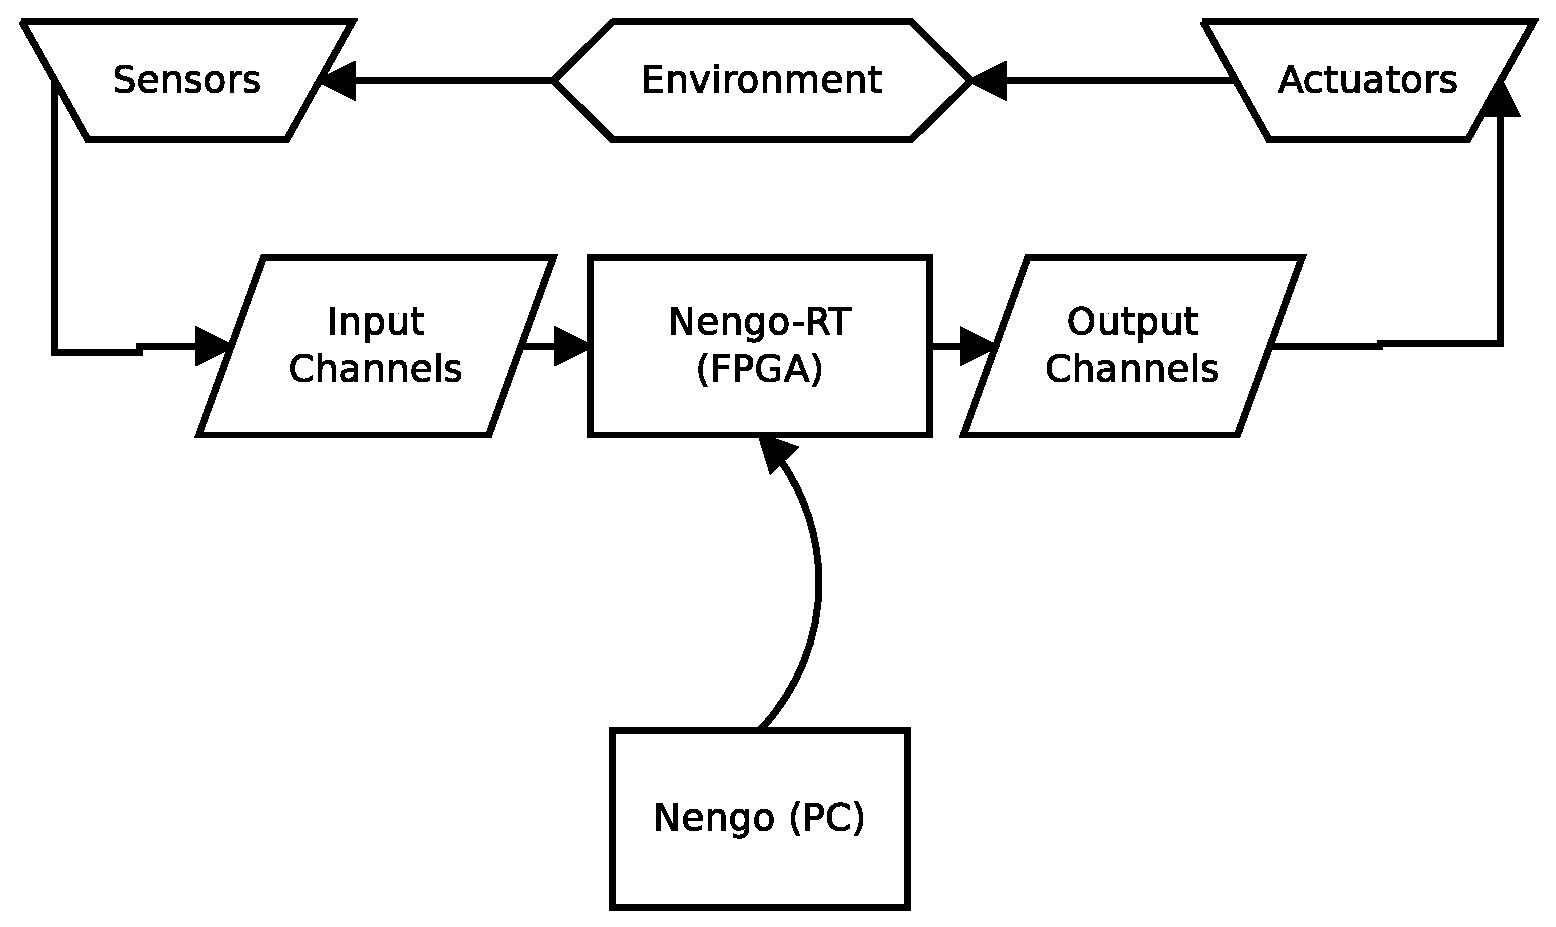
\includegraphics[width=5.0in]{robot-closed-loop.eps}

\caption{Block diagram of a high-level closed-loop autonomous system using \design{}.}
\label{fig:closedloop}
\end{figure}

The top-level module exposes a programming interface that allows for any of the runtime configurable components
(decoded value buffers, encoders, population unit filters, principal component lookup tables,
population unit noise generators, decoder vectors, and I/O channels) to be initialized and programmed
over an external interface such as Ethernet. This allows a single implementation of the design
to be used to simulate a large number of different neural networks without requiring modifications to the physical hardware.
The programming interface also allows an external controller to reset the hardware and to start, pause, or single-step a simulation
without requiring physical access to the hardware.

\subsection{Constraints on models}

There is a limitation on the complexity of the encoding operation due to the length of the instruction buffer that is used.
Because each encoder must produce 1024 encoded values per timestep, using an instruction memory of size 8192 for each encoder means that a maximum of eight decoded values
can be used as input to each encoder per population.
If a higher fan-in is required, the hardware design could be modified to allocate more memory to the instruction buffers,
which in turn would reduce the amount of memory available for other portions of the design.
It is theoretically possible to simulate populations that require more than eight decoded values to be read by a single encoder
without increasing the size of the instruction buffers,
but the extra instructions used for this mean that other populations sharing that encoder will have to use fewer.
The compiler can detect this scenario and reorganize populations appropriately so as to avoid overfilling the instruction buffers.

As only one-dimensional and two-dimensional population units have been implemented, networks that require populations to compute functions
of three or more independent variables cannot be simulated with this design.
However, the majority of existing models in Nengo do not use populations with more than two input dimensions.
A controlled oscillator is an example of a kind of NEF network that cannot be simulated in our hardware implementation,
because it requires the approximation of a three-dimensional nonlinear function. Our implementation can simulate higher-dimensional representations
by simulating dimensions individually or in pairs, as long as each approximated function is either linear or is nonlinear in only one or two dimensions.

The choice of using a maximum of four sets of decoder vectors per population is arbitrary; it seems to be a good balance between
population connectivity and memory usage. Populations that have more than four outgoing connections must be treated specially.
Assuming none of the outgoing connections can be combined together (for example, if the function they decode only differs by a constant),
in order to implement such a population on the simulator, it is necessary to duplicate it and simulate it
$n/4$ times, once for each group of up to four decoder vectors.
The consequence of this is that a population with more than
four outgoing connections will be represented as two or more populations in simulation, thereby reducing the actual number of
distinct populations that can be simulated.

\subsection{Implementation details}

A hardware implementation of the \design{} design was produced on a Xilinx VC707 development board, which includes a modern field-programmable gate array (FPGA)
device (Xilinx XC7VX485T-2FFG1761C). This device was chosen because of its ready availability on a development platform and its large logic capacity and available resources.
In particular, it provides 37080~Kb of on-chip block RAM and 2800 customizable DSP slices, both of which the Nengo-RT design requires in abundance in order to support
the largest possible implementation size. 

% FIXME implemented design size

The implemented hardware operates at a clock speed of 125~MHz, using the same external clock source as the Gigabit Ethernet transceiver.
This is convenient as it means that the entire design, including both the simulator hardware and the I/O interfaces, operates from the same clock source.
Because of this, there is no latency when receiving input or transmitting output to and from the simulation;
if two different clock speeds were used, extra buffers would have to be implemented in order to ``cross'' the two clock domains,
and the logic operating in the faster clock domain would occasionally have to wait for the slower-clocked logic to consume input from the buffer.
This type of stall would prevent part of the simulator from operating in real-time; by using the same clock for all logic, however, this problem is averted and
both input and output are wait-free.

The VC707 development board provides a Gigabit Ethernet transceiver that can be used for fast off-board communication to a PC.
A simple Ethernet stack was implemented as part of the Nengo-RT design to expose a programming interface to the Nengo software,
as well as to provide input and output of decoded values during simulation.

% FIXME maximum channel capacity in terms of decoded values

\subsection{Nengo backend}

% FIXME quick description of Nengo
Nengo's ensembles of neurons become populations that are simulated in the hardware on population units.
Connections between populations are handled through encoders and decoders.
Nodes and probes, which collect data or evaluate arbitrary functions in software, are
simulated on the host computer and are transferred to and from the board over hardware 
I/O channels after every timestep. 
By default, the hardware operates in real-time; the software receives new output data from the board
every millisecond and is responsible for processing this data and sending new inputs back to the hardware as quickly as possible.
The software does not have to send inputs for every timestep; if no new data is sent, the old values will be preserved.
This means that more work can be done in software while still operating the hardware in real-time by, for example,
only computing new input values every fifth timestep.
If strict synchronization is necessary, or if real-time operation is not possible,
the hardware can be run in a single-step mode, which forces it to pause after completing each timestep in order
to allow the software time to complete its tasks, which may include updating plots, logging received data to a file,
computing node functions, and calculating and sending new input values to the hardware.
This mode of operation, while not real-time, makes it possible to run hardware-assisted simulations
on a slower PC or when the software component is too complex or slow to be performed in sync with the hardware
(for example, logging a large number of decoded values to a hard drive).

A backend to Nengo performs the task of compiling a Nengo model to a loadfile that can be
simulated on the hardware. The compiler calculates principal components for each population
of neurons, and then performs a clustering operation in order to associate many
populations with each set of principal components while minimizing the differences
between the approximate principal components and the actual values. % FIXME explain/calculate why actual principal components cannot be used
The compiler calculates decoders and encoders for each population with respect
to the shared principal components, and computes an optimized encoder schedule % FIXME details needed here
that coordinates reads made by each encoder so that all operations can be performed
in as few clock cycles as possible while avoiding a read collision on any decoded value block.
Once the compiler has finished writing out the loadfile, the Nengo simulator
transfers the configuration data to the hardware and controls input and output during the simulation.

% clustering algorithm, quantization error for large populations -- this needs its own section

\section{Results}

% integrator (1d)
% oscillator (2d)
% feed-forward nonlinear functions
% 2D multiplication

% scope of situations for which it works well
% full neurons vs. CPU populations vs. hardware populations
% high-frequency breakdown (square wave, sinusoids)
% qualitative comparison: show the figure, talk about the figure
% possible quantitative approach (RMSE)

% hardware-specific results: how many populations, 
% circumstances under which an overflow could occur
% (probabilistic analysis), power analysis,
% resource utilization

% FIXME may need a simpler example first -- just an input driving an identity population from 0 to 0.5 in steps of 0.1. This is good for contrast.

To verify the correct operation of the hardware as well as the software backend to Nengo, a simple network consisting of a single neural integrator was compiled and simulated on the hardware.
Figure~\ref{lst:integrator1d} shows the code listing and the resulting network that it describes.
\begin{figure}
\centering

\begin{subfigure}[b]{\textwidth}
\centering
\lstset{language=Python}
\begin{lstlisting}[frame=single]
import nengo
import nengo.helpers
model = nengo.Model(label='Integrator')
input = nengo.Node(nengo.helpers.piecewise({0:0.5}), label='Input')
tau = 0.1
A = nengo.Ensemble(nengo.LIF(100, tau_rc=0.02, tau_ref=0.002,
                   dimensions=1, label='Integrator'))
nengo.Connection(A, A, transform=[[1]], filter=tau)
nengo.Connection(input, A, transform=[[tau]], filter=tau)
p1 = nengo.Probe(input, 'output')
p2 = nengo.Probe(A, 'decoded_output', filter=0.01)
\end{lstlisting}
\caption{Source code}
\label{lst:integrator1d:code}
\end{subfigure}

\begin{subfigure}[b]{0.3\textwidth}
\centering
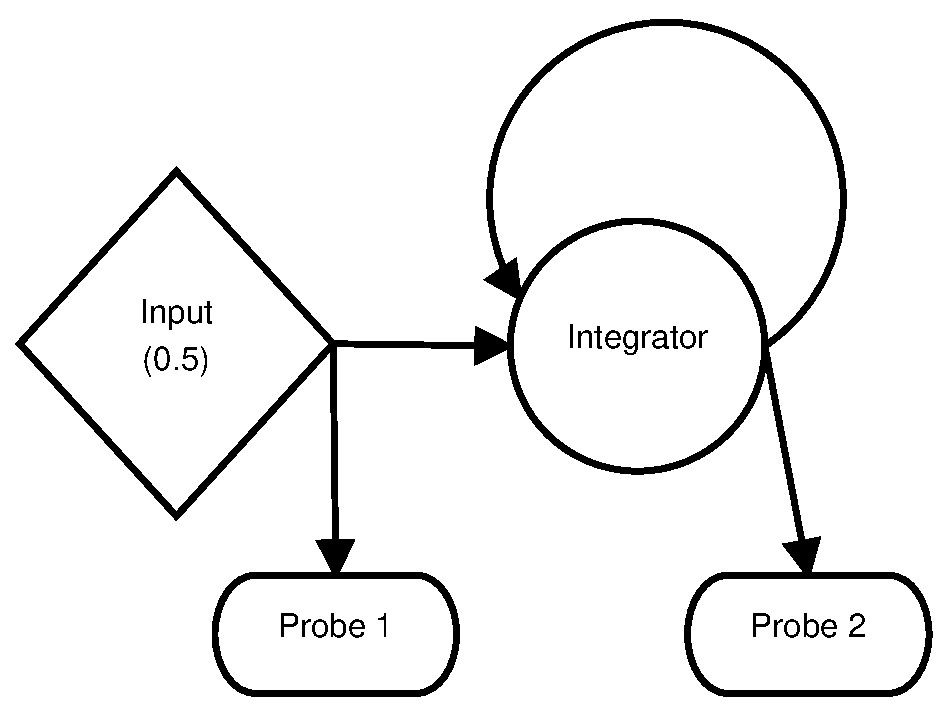
\includegraphics[width=3.0in]{integrator-1d-schematic.eps}
\caption{Schematic}
\label{lst:integrator1d:schematic}
\end{subfigure}

\caption[A 1D neural integrator in Nengo.]
{Source code (\ref{lst:integrator1d:code}) and schematic (\ref{lst:integrator1d:schematic}) of a 1D neural integrator in Nengo.}
\label{lst:integrator1d}
\end{figure}

% FIXME explanation of the code?
The network was compiled with the \design{} backend to produce a programming file that could be used to configure the simulator hardware.
Simulation output from the FPGA was captured with an Ethernet traffic sniffer and plotted in Figure~\ref{fig:integrator1d}.

\begin{figure}
\centering

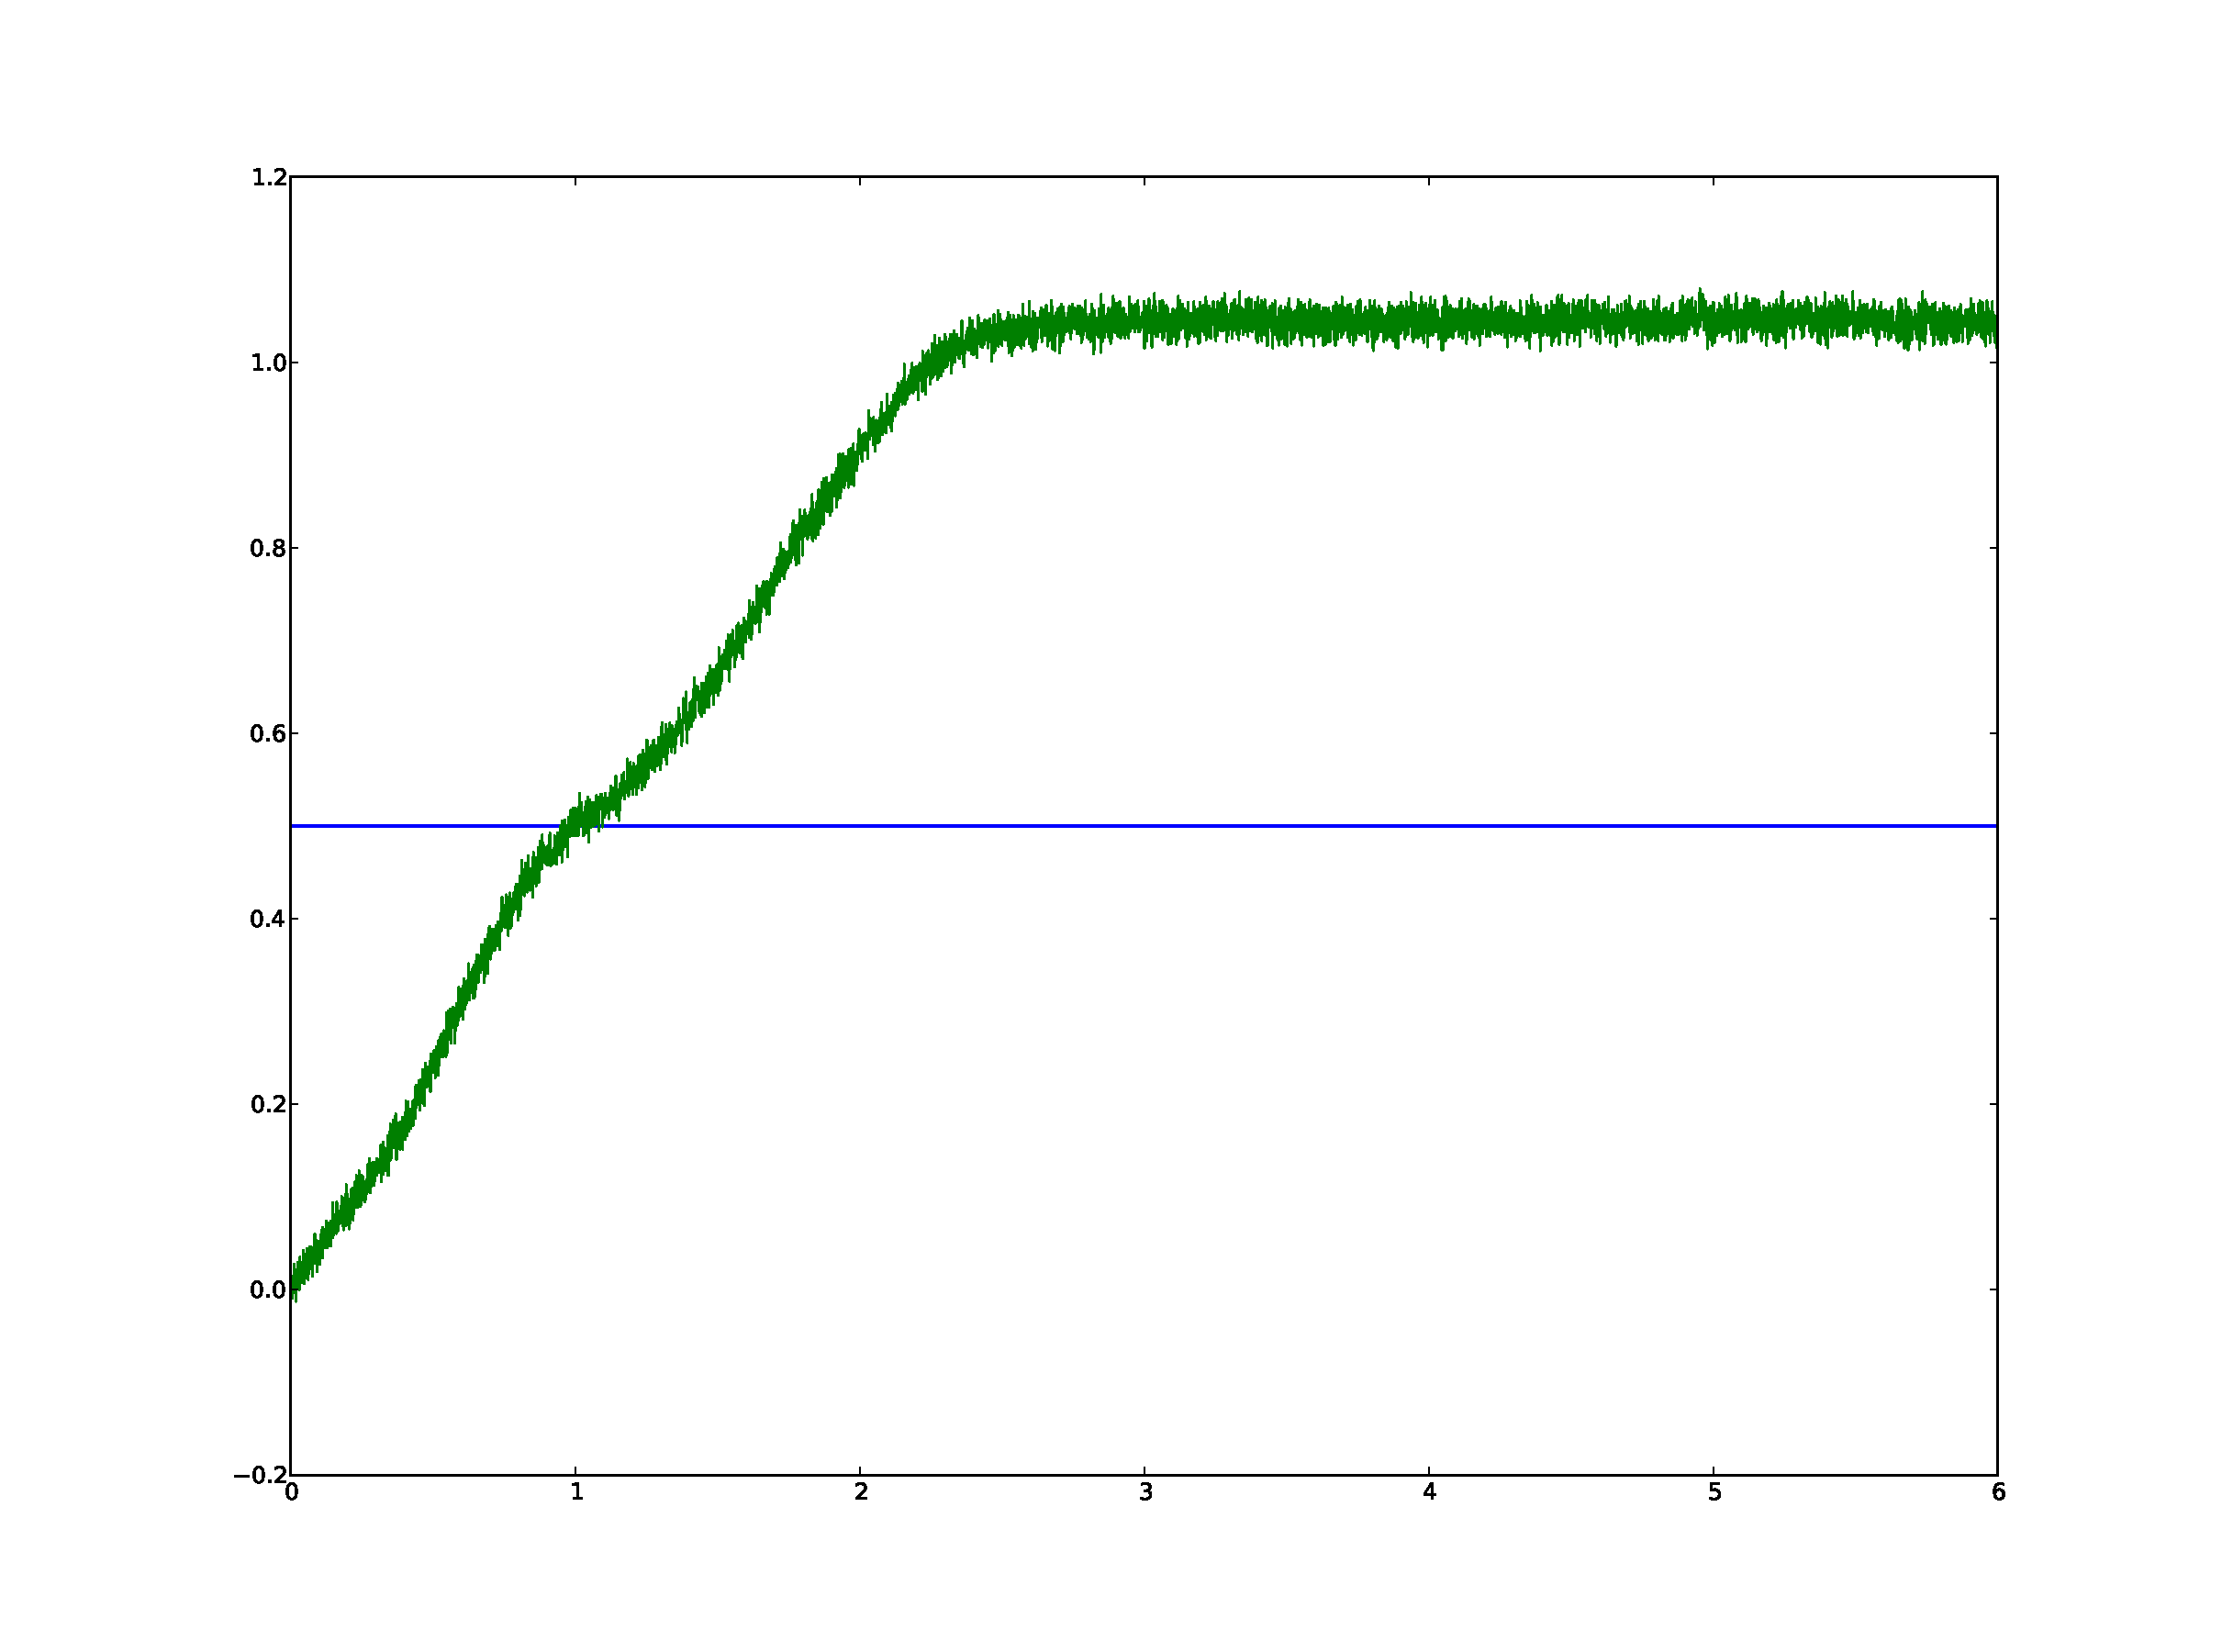
\includegraphics[width=6in]{integrator-1d.eps} % FIXME software plot
% FIXME figure: larger axis and label font, make this consistent across all figures

\caption[Simulation of a 1D neural integrator.]
{Hardware output from simulation of a one-dimensional population representing a neural integrator.}

\label{fig:integrator1d}
\end{figure}

Given a constant input value of 0.5, the output from the integrator approaches this value
over time and reaches it after 1.0 seconds, then continues to accumulate the input until
another second has elapsed. The population saturates and remains at 1.0 after this time
because it is not able to represent values with a magnitude greater than 1.0. However,
the integrator's behaviour for the first two seconds of simulation is correct and confirms
the proper operation of the one-dimensional population hardware.

The two-dimensional population unit was tested with a simple single-population van der Pol oscillator.
Figure~\ref{lst:oscillator2d} shows the code listing and the network generated in Nengo;
Figure~\ref{fig:oscillator2d} shows output from the \design{} hardware simulation.

\begin{figure}
\centering

\begin{subfigure}[b]{\textwidth}
\centering
\lstset{language=Python}
\begin{lstlisting}[frame=single]
import nengo
import nengo.helpers
model = nengo.Model('Oscillator')
neurons = nengo.Ensemble(nengo.LIF(200), dimensions=2, 
  label='van der Pol Oscillator')
input = nengo.Node(output=nengo.helpers.piecewise(
  {0:[1,0], 0.1:[0,0], label='Initial condition')
tau = 0.1
freq = 5.0
input2output = nengo.Connection(input, neurons)
recurrent = nengo.Connection(neurons, neurons, 
  transform=[[1, -freq*tau],[freq*tau,1]], filter=tau)
input_probe = nengo.Probe(input, 'output')
neuron_probe = nengo.Probe(neurons, 'decoded_output', filter=0.005)
\end{lstlisting}
\caption{Source Code}
\label{lst:oscillator2d:code}
\end{subfigure}

\begin{subfigure}[b]{0.3\textwidth}
\centering
% FIXME \includegraphics[width=3.0in]{oscillator-2d-schematic.eps}
\caption{Schematic}
\label{lst:oscillator2d:schematic}
\end{subfigure}

\caption[A 2D neural oscillator in Nengo.]
{Source code (\ref{lst:oscillator2d:code}) and schematic (\ref{lst:oscillator2d:schematic})
of a 2D neural oscillator in Nengo.}
\label{lst:oscillator2d}
\end{figure}

\begin{figure}
\centering
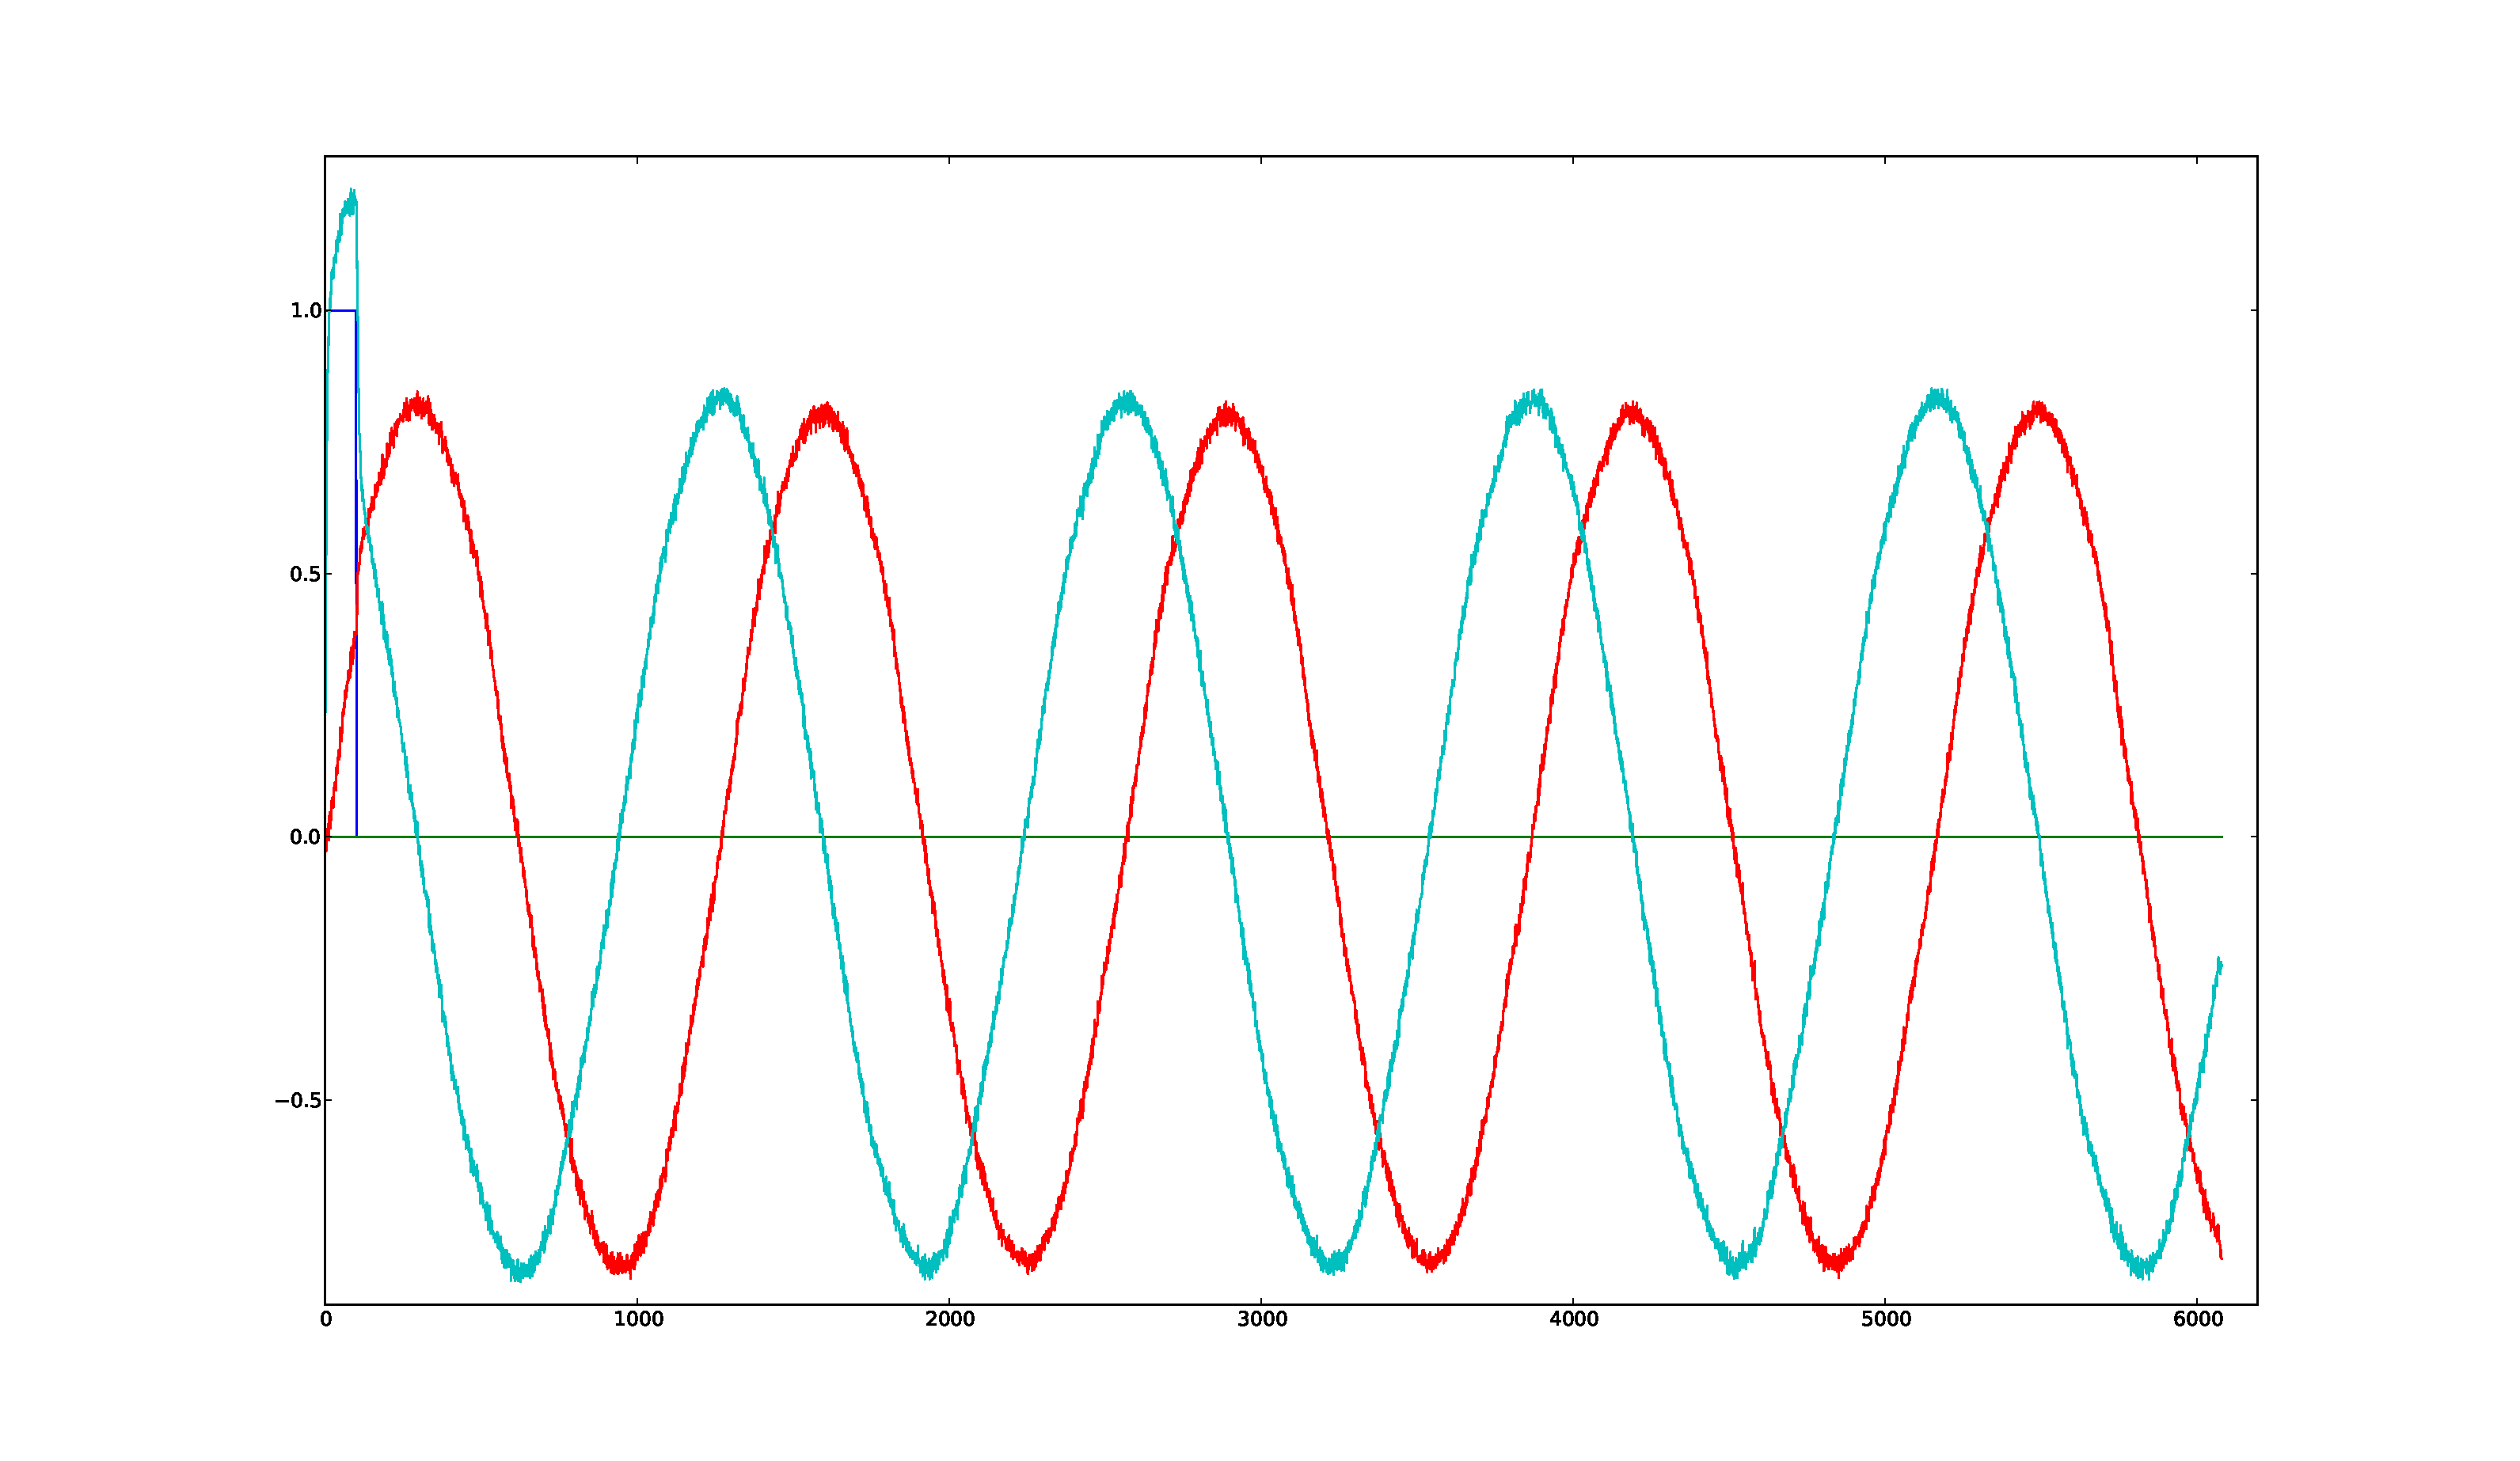
\includegraphics[width=6in]{oscillator-2d.eps}

\caption[Simulation of a 2D neural oscillator.]
{Hardware output from the simulation of a two-dimensional population representing a neural oscillator.}
\label{fig:oscillator2d}
\end{figure}

The oscillator requires a brief non-zero ``start-up'' input in order to begin oscillating.
After this input disappears (0.1~s), both dimensions of the decoded output can be seen to
oscillate in a sinusoidal fashion. This oscillation, once started, will proceed indefinitely.
% FIXME frequency analysis?
The oscillation as observed in the figure confirms the correct operation of the two-dimensional
population hardware.

As a test of a combined network with both one-dimensional and two-dimensional populations,
a neural multiplier was simulated on the hardware. Figure~\ref{lst:multiplier} shows
the code listing and the resulting network that it describes.

\begin{figure}
\centering

\begin{subfigure}[b]{\textwidth}
\centering
\lstset{language=Python}
\begin{lstlisting}[frame=single]
import nengo
import nengo.helpers
model = nengo.Model('Multiplier')
A = nengo.Ensemble(nengo.LIF(100), dimensions=1,
  radius=1.4, label='A')
B = nengo.Ensemble(nengo.LIF(100), dimensions=1,
  radius=1.4, label='B')
combined = nengo.Ensemble(nengo.LIF(224), dimensions=2,
  radius=2, label='combined')
prod = nengo.Ensemble(nengo.LIF(100), dimensions=1,
  radius=2, label='prod')

inputA = nengo.Node(nengo.helpers.piecewise
  ({0:0, 2.5:0.5, 4:-0.5}))
inputB = nengo.Node(nengo.helpers.piecewise
  ({0:1.0, 1.5:0.8, 3:0.0, 4.5:0.8}))

nengo.Connection(inputA, A)
nengo.Connection(inputB, B)

nengo.Connection(A, combined, transform=[[1],[0]])
nengo.Connection(B, combined, transform=[[0],[1]])

def product(x):
  return x[0] * x[1]

nengo.Connection(combined, prod, function=product)

A_probe = nengo.Probe(A, 'decoded_output', filter=0.01)
B_probe = nengo.Probe(B, 'decoded_output', filter=0.01)
prod_probe = nengo.Probe(prod, 'decoded_output', filter=0.01)
\end{lstlisting}
\caption{Source code}
\label{lst:multiplier:code}
\end{subfigure}

\begin{subfigure}[b]{0.3\textwidth}
\centering
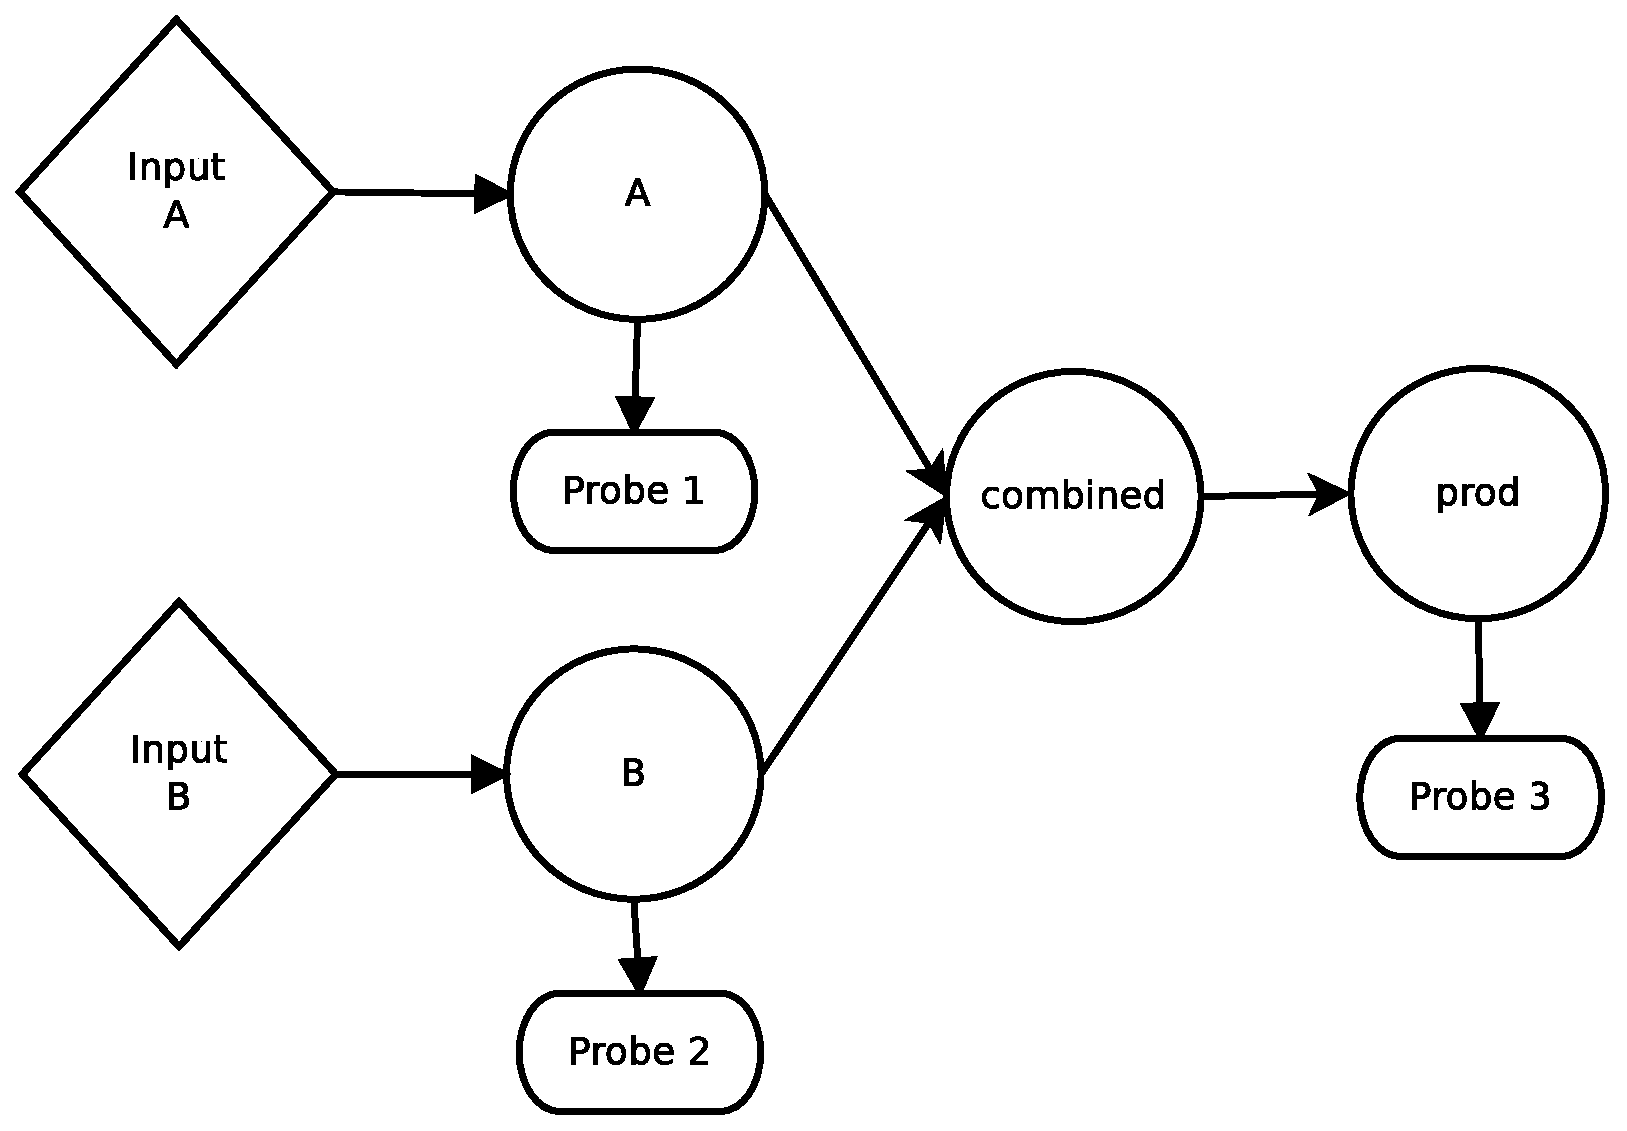
\includegraphics[width=3.0in]{multiplier-schematic.eps}
\caption{Schematic}
\label{lst:multiplier:schematic}
\end{subfigure}

\caption[A multiplier in Nengo.]
{Source code(\ref{lst:multiplier:code}) and schematic (\ref{lst:multiplier:schematic})
of a multiplier in Nengo.}
\label{lst:multiplier}
\end{figure}

% FIXME: explain input and expected output

Simulation of this network in hardware produced results comparable to those obtained in software
(Figure~\ref{fig:multiplier}).

\begin{figure}
\centering

% FIXME change the bounds on the axes to make it easier to see the similarities

\begin{subfigure}[b]{0.5\textwidth}
\centering
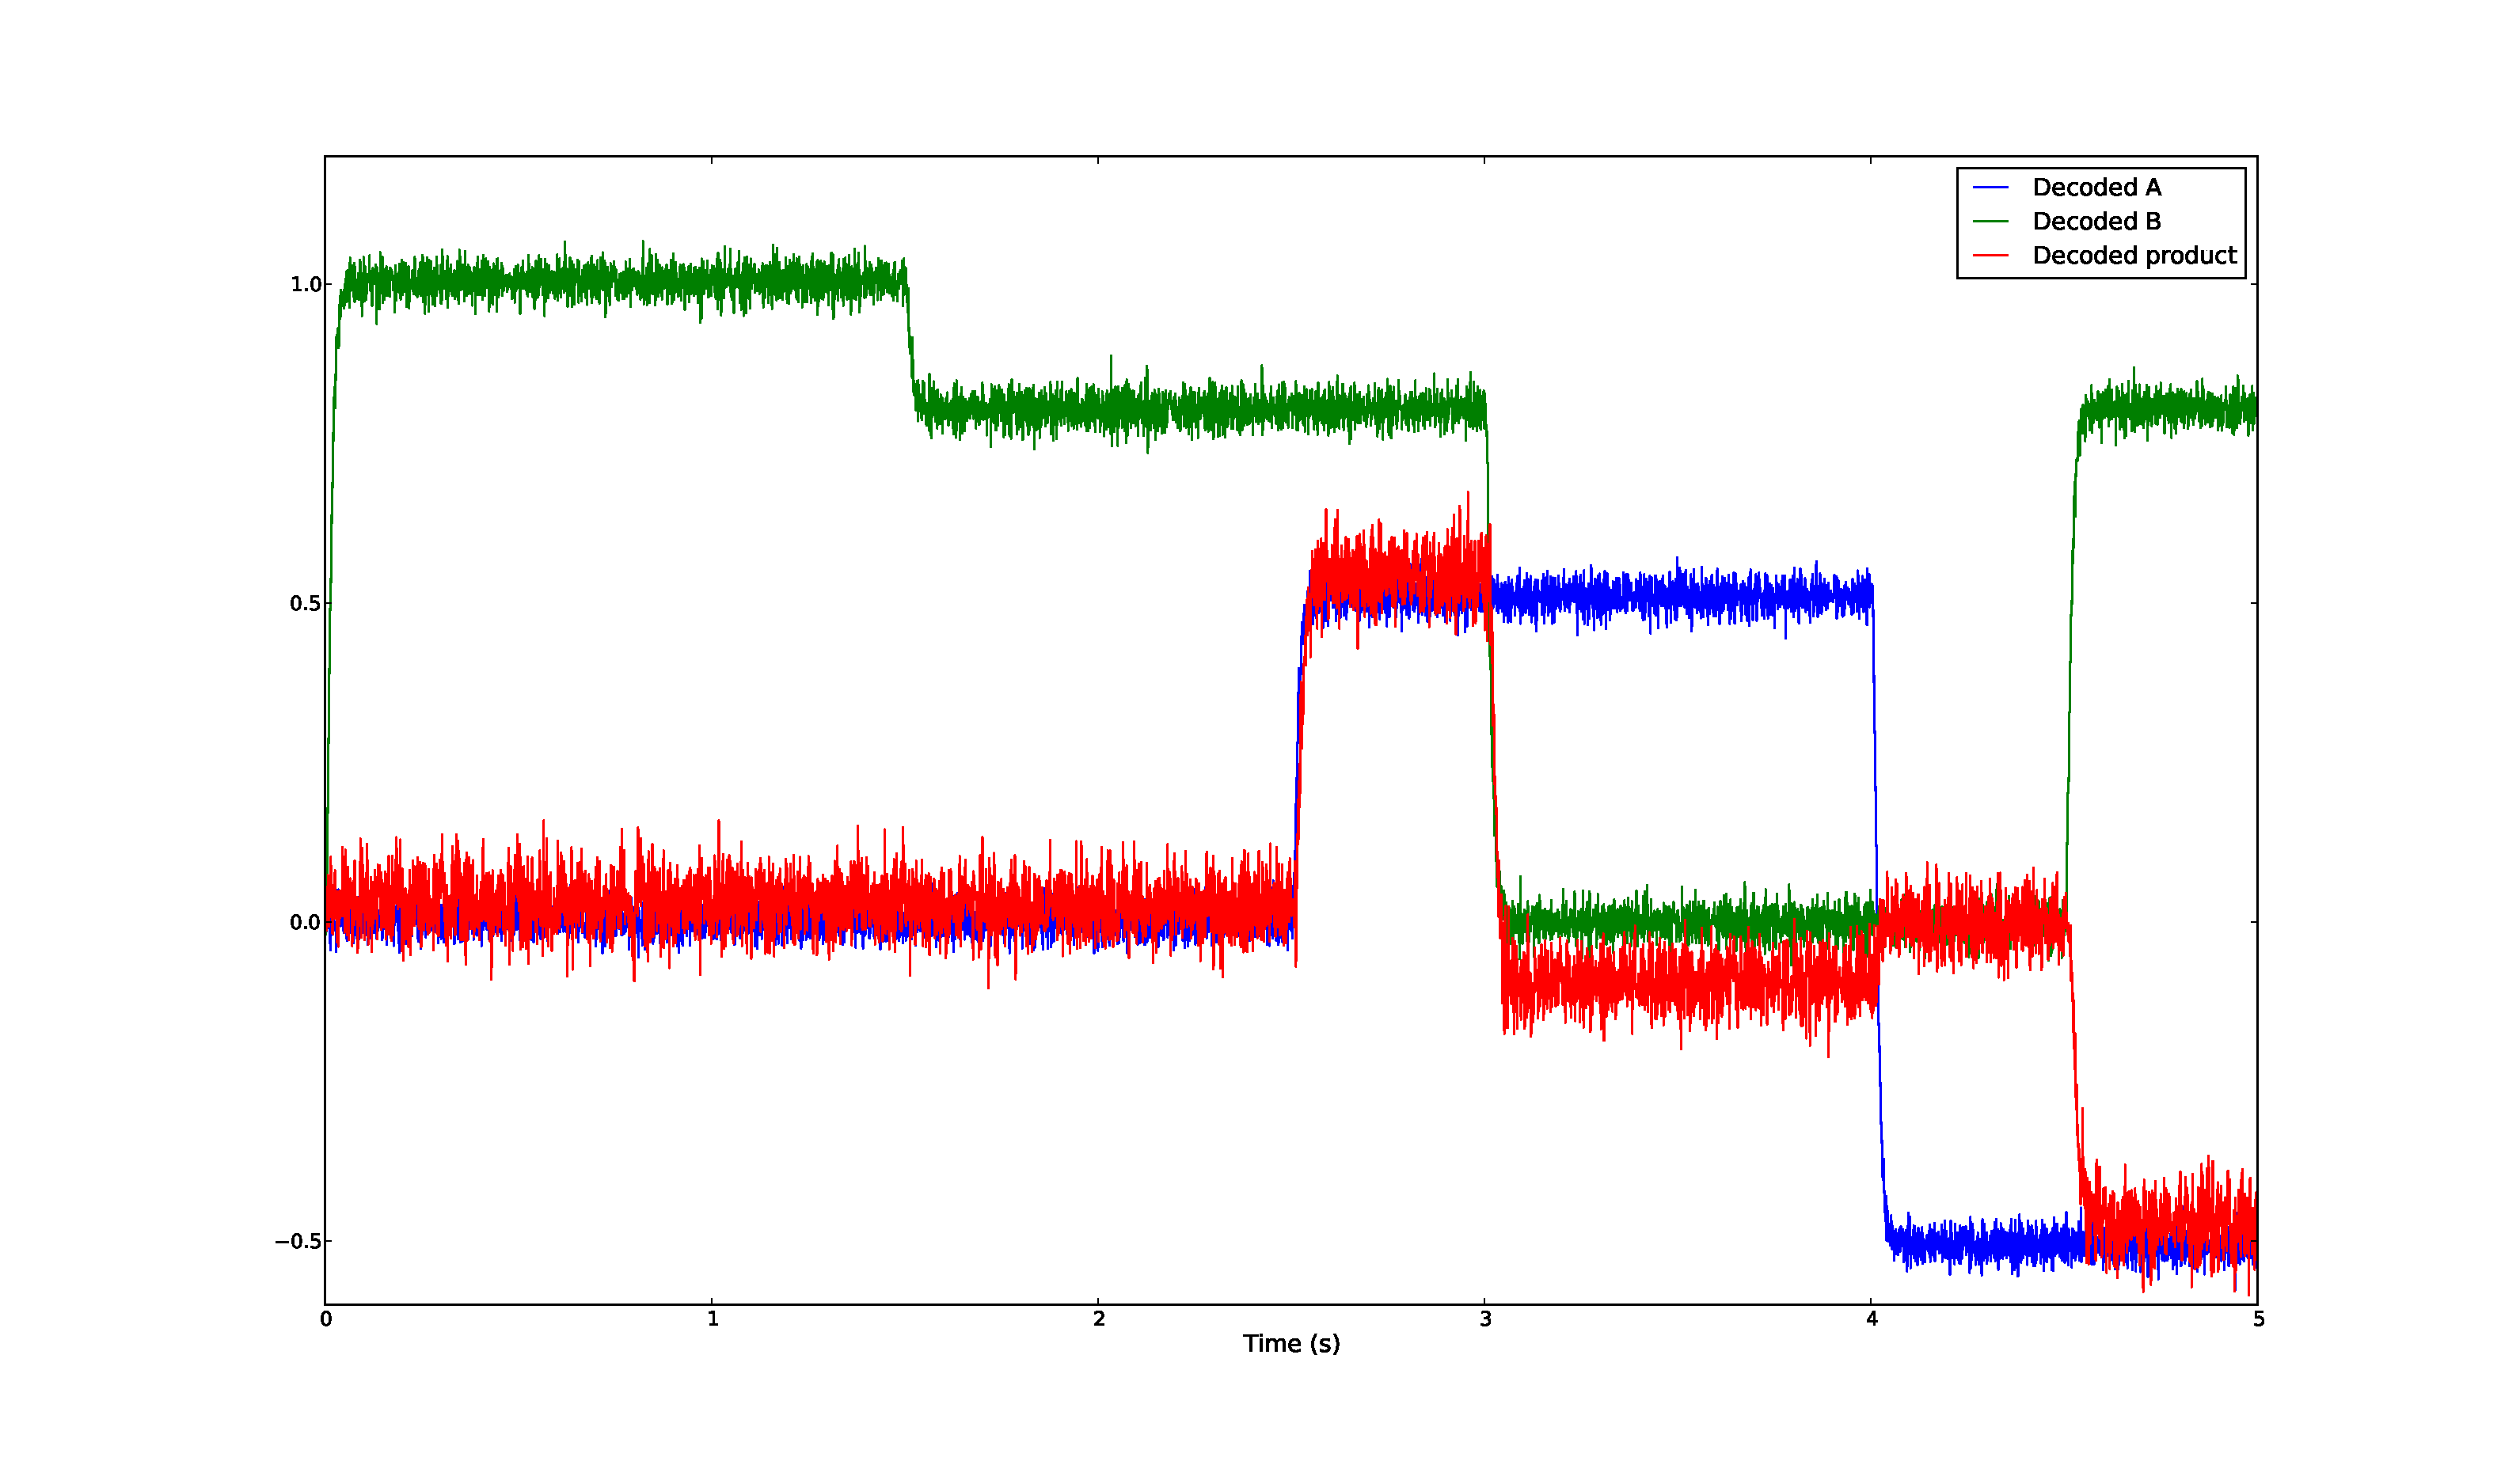
\includegraphics[width=3in]{multiplier-sw.eps}
\caption{Software}
\label{fig:multiplier:sw}
\end{subfigure}

\begin{subfigure}[b]{0.5\textwidth}
\centering
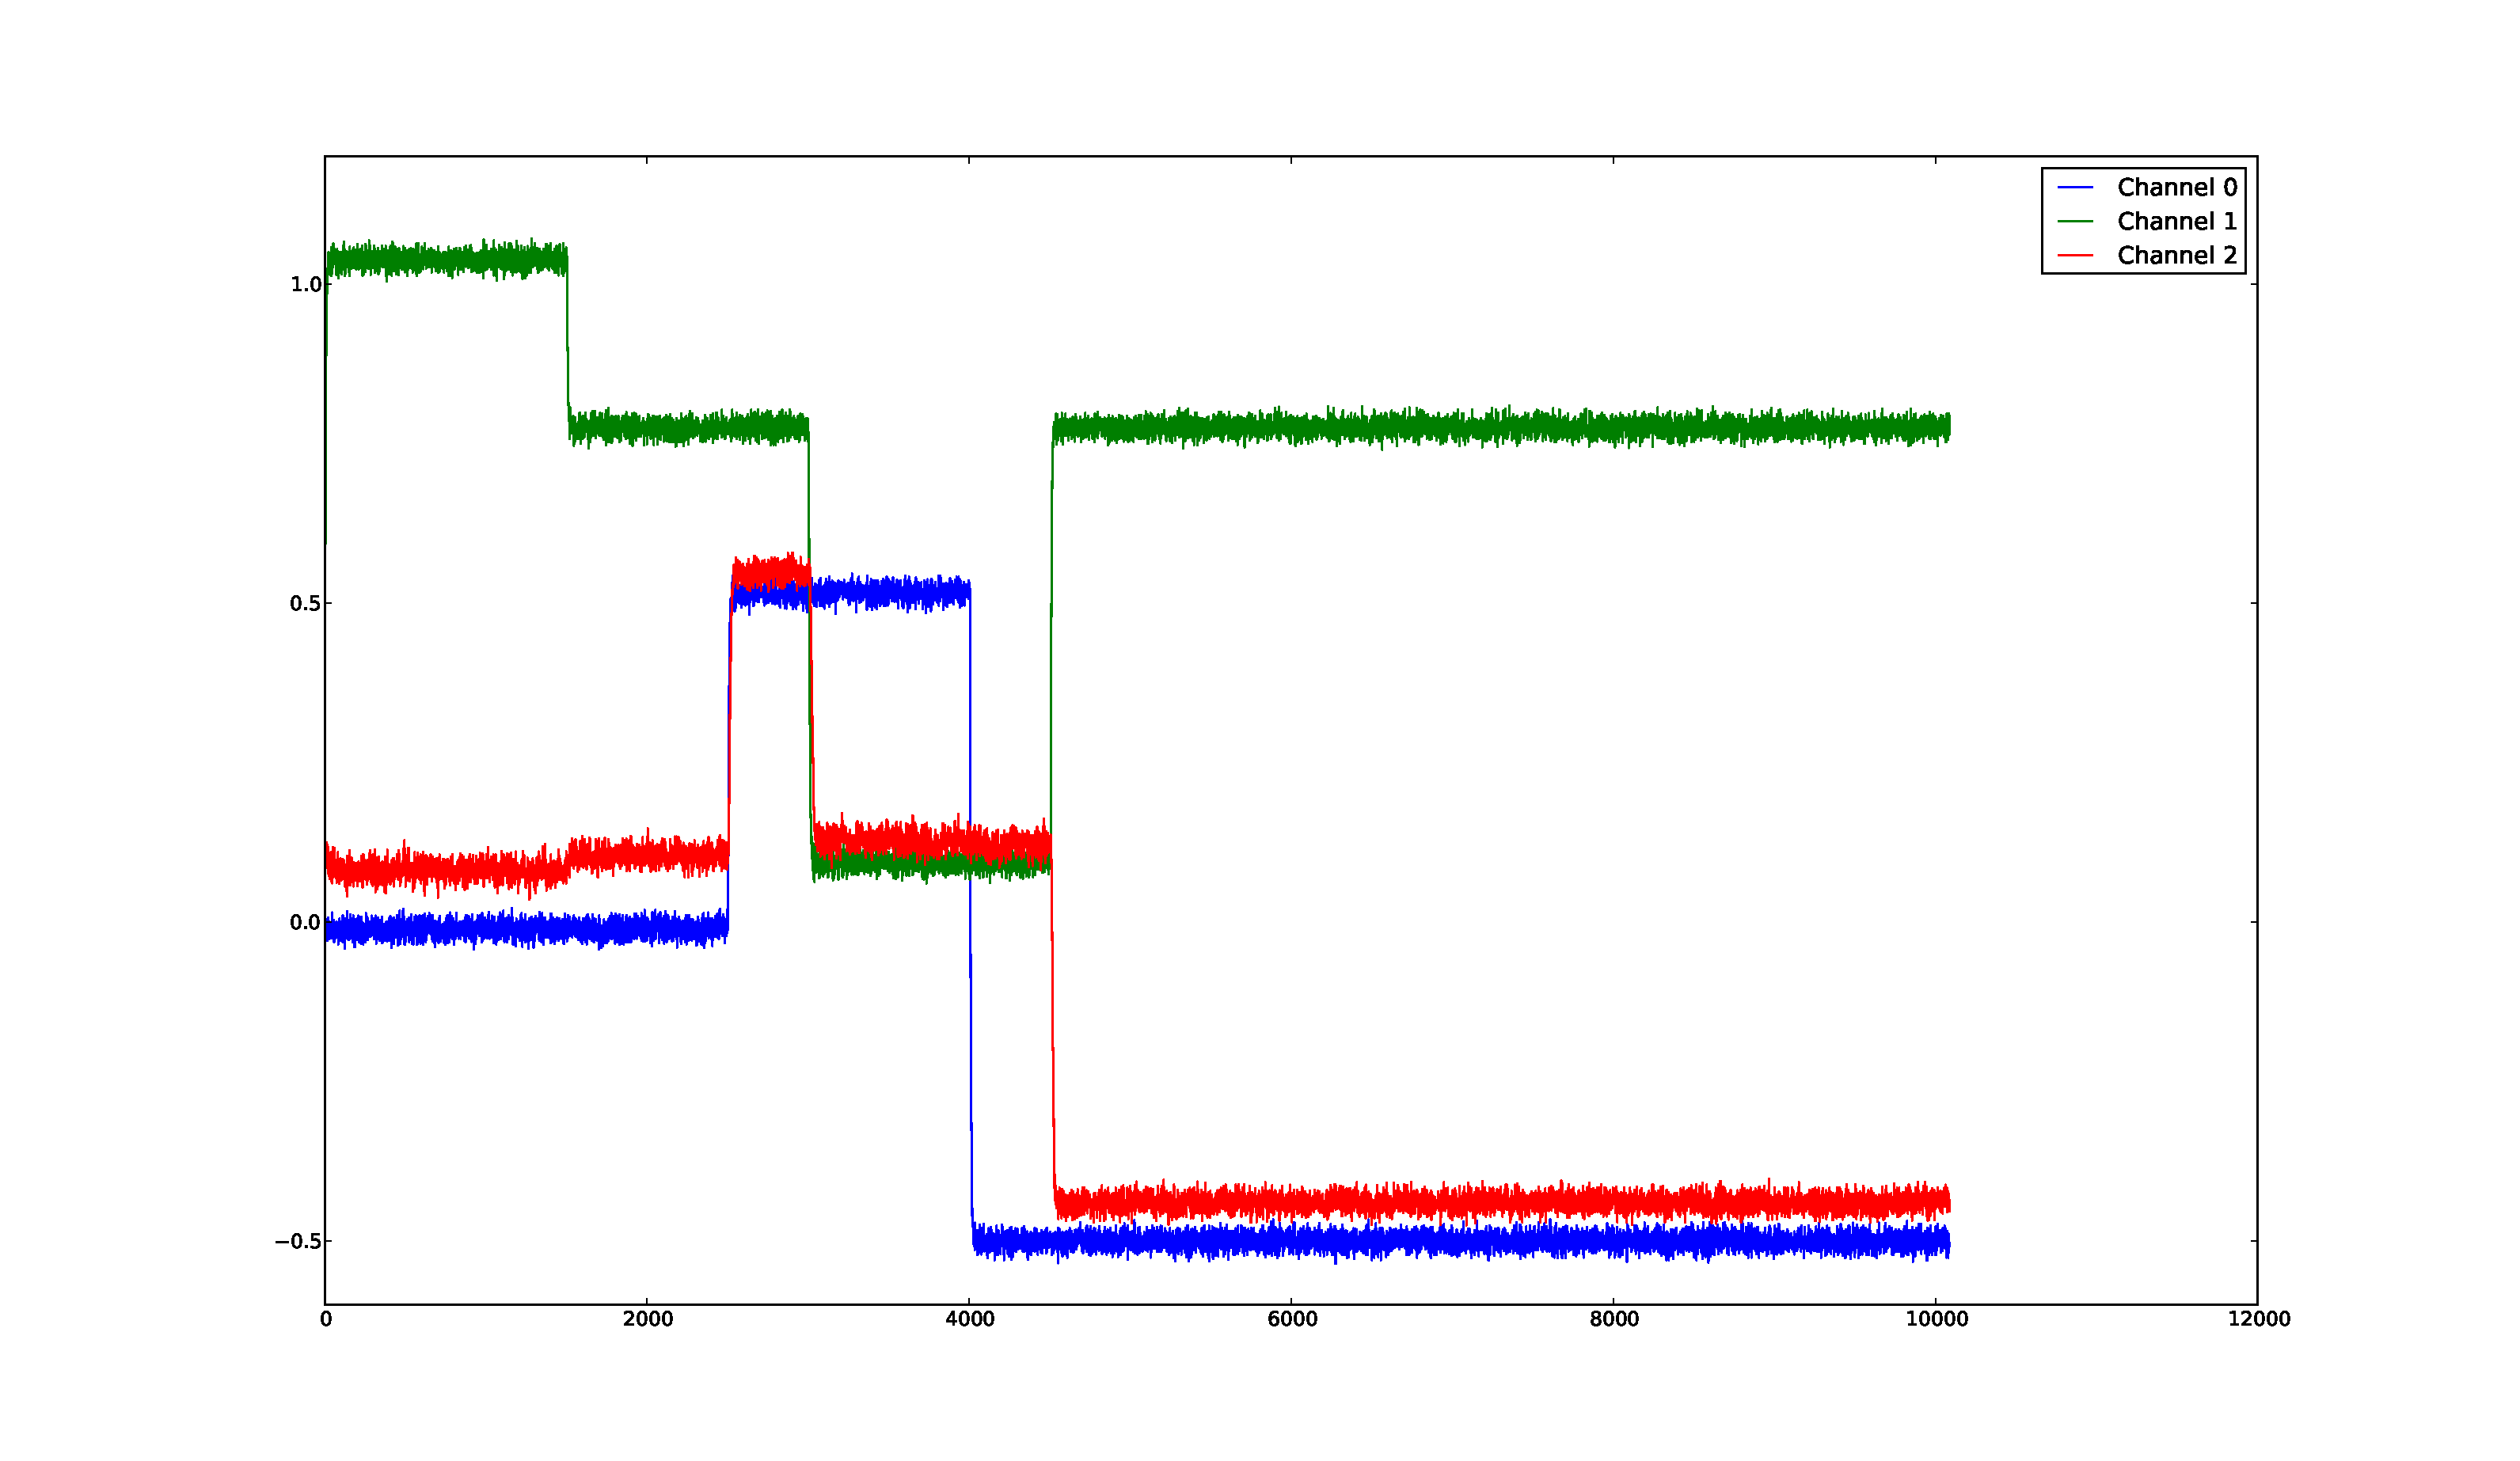
\includegraphics[width=3in]{multiplier.eps}
\caption{Hardware}
\label{fig:multiplier:hw}
\end{subfigure}

\caption[Multiplier simulation comparison.]
{Comparison of software (\ref{fig:multiplier:sw}) and hardware (\ref{fig:multiplier:hw})
simulation of a neural multiplier network.}
\label{fig:multiplier}
\end{figure}

\subsection{power, \% timestep used for each simulation, \% of board resources for each simulation}

\section{Discussion}

\subsection{How well it worked}

\subsection{Limitations}

Our current implementation does not support populations that represent variables of three or more dimensions.
Support for higher-dimensional populations could be added in the future.
However, as the number of dimensions increases, the
amount of memory that must be used to store principal components and
decoders increases as well; therefore, beyond a certain number of
dimensions it would become impractical to implement a hardware
population unit.  

Nengo supports a more advanced connection called a learning connection,
which mdoifies the decoders of a population according to a particular ``learning rule''
as a function of other represented values. The hardware design does not support this special connection type.
It was decided to implement the most common cases first in order to demonstrate the feasibility of simulating
neural networks in population mode on the hardware, and since many networks do not use learning connections,
support for them was omitted from this version.

Most connections in Nengo have both positive and negative synaptic weights. This
structure is meant as a simplified model of a common excitatory/inhibitory circuit
(Parisien et al.) % FIXME citation
Nengo also has a special kind of connection called an inhibitory connection that
reduces activity in all neurons of the target population. We did not model this kind of connection explicitly.
However, such a connection onto a 1D population could be modelled by treating the population as 2D,
setting the second element of each neuron's encoder to -1, and connecting inhibitory inputs to this dimension.

% high-frequency stuff (this will depend on other results)

\subsection{Future work \& extensions}


The flexibility of input and output channels lends to their use in connecting multiple devices together for use as part of a larger simulation engine.
This would allow networks to be simulated that consume more resources than are available on a single device, which may in turn allow
for ``grids'' of inexpensive hardware devices to be used to simulate a very large model.

The current control and I/O interface communicates over Ethernet, but since bare frames are being used with no higher-level protocols on top of them,
it is somewhat cumbersome to set up a computer or other device to send and receive data to the hardware.
This approach is suitable for testing and prototyping, but it makes certain assumptions about the setup of the network and the host computer that
may not be reasonable for general use, such as requiring raw socket privileges on the host operating system (which typically require administrator access).
A more user-friendly approach would be to implement an Ethernet stack that supports a protocol such as UDP, which can be readily used by many different
kinds of host software in order to interact with a simulation.

At present, the interconnect between the encoders and the decoded value
buffers is the most complex part of the design in terms of the density of its logic
in hardware. If there are $N$ encoders and $M$ decoded value buffers, a total of
$NM$ connections must be made between these components in order for every
encoder to be able to read from every decoded value buffer.
Note that this is still a massive improvement over a neuron-to-neuron interconnect,
which would require over 10000 times as many connections to provide all-to-all connectivity.
% FIXME contrast this with size of neuron-to-neuron interconnect
For large numbers
of encoders and decoded value buffers, the complexity of the interconnect at
that design size makes it impossible for the FPGA design tools to find a way to
implement that part of the design on the device. This is currently the limiting
factor in terms of the number of population units that can be implemented on
the development board (as opposed to, for example, a lack of memory blocks for
decoded value buffers). A future version of the \design{} design may address
this issue and implement an interconnect that scales well to larger numbers of
encoders and decoded value buffers in order to allow more populations to be
simulated. % FIXME how could this be done?

\end{document}
